% =============================================================================
\bloco{1}{Exam level: Benigno's own experiments, Lista 7 and Carlin--Soskice}{Benigno \S\S6, 7, 11 \,\textbullet\, 40 points}

\questao{(10 points) \textit{Source: built on Benigno, P. (2015), ``New-Keynesian Economics: An AS--AD View'', \S6.1--\S6.2,
Figs.~6--7, p.~512 --- the article has no exercises; the statement below is ours. The article treats a productivity \emph{gain};
here the sign is reversed.}
Redo the two experiments of those sections for a productivity \emph{fall}, $da<0$.}

\noindent What the article states (p.~512): ``First, we analyze the case in which the economy undergoes a temporary productivity
gain, meaning that productivity rises in the short run but does not vary in the long run.'' (\S6.1) and ``Fig.~7 analyzes the case
of a permanent productivity shock.'' (\S6.2)

\textbf{a)} (4 points) The fall is temporary ($d\bar a=0$) and $i$ stays at its initial level. Which curve moves, in which direction and
why? Find $dy$, $dp$, $d(y-y_n)$ and $d(y-y_e)$ in closed form, with signs.
\resolespaco
\begin{sol}
\begin{notacao}
\item $y$, $p$: log output and log price level today. $\bar y$, $\bar p$: their long-run values ($\bar p$ fixed throughout).
\item $p^e$: the price preset by the firms that cannot adjust this period (fixed unless stated).
\item $y_n$: natural output (flexible prices, with the markup), \eqref{YN}. $y_e$: efficient output (no markup), \eqref{YE}.
$y-y_n$ and $y-y_e$: the two output gaps.
\item $i$: nominal interest rate, the bank's instrument. $\rho\equiv-\ln\beta>0$, with $\beta\in(0,1)$ the discount factor.
\item $a$, $\bar a$: productivity today and in the long run. $\mu$, $\bar\mu$: desired markup today and in the long run.
$g$, $\bar g$: public spending today and in the long run.
\item $\sigma>0$: intertemporal elasticity of substitution. $\eta>0$: inverse Frisch elasticity. $\kappa>0$: slope of \eqref{AS}.
$\Omega\equiv\sigma^{-1}+\eta>0$.
\item $d(\cdot)$: the change of a variable from the initial efficient steady state. Here $da<0$ and $d\bar a=0$.
\item (M): the gap equation derived in the first step; every later question of the list uses it.
\end{notacao}
\passo{the machine}{$\ln\beta$ is a constant. Differentiate \eqref{AD}:}
\begin{equation}
dy=d\bar y+dg-d\bar g-\sigma\,di+\sigma\,d\bar p-\sigma\,dp. \label{q1:dAD}
\end{equation}
Differentiate \eqref{AS}:
\begin{equation}
dp=dp^e+\kappa\,(dy-dy_n). \label{q1:dAS}
\end{equation}
Substitute \eqref{q1:dAS} for $dp$ in \eqref{q1:dAD}:
\begin{align}
dy&=d\bar y+dg-d\bar g-\sigma\,di+\sigma\,d\bar p-\sigma\big(dp^e+\kappa\,(dy-dy_n)\big)\nonumber\\
&=d\bar y+dg-d\bar g-\sigma\,di+\sigma(d\bar p-dp^e)-\sigma\kappa\,dy+\sigma\kappa\,dy_n . \nonumber
\end{align}
Move $-\sigma\kappa\,dy$ to the left side:
\begin{equation}
(1+\sigma\kappa)\,dy=d\bar y+dg-d\bar g-\sigma\,di+\sigma(d\bar p-dp^e)+\sigma\kappa\,dy_n . \label{q1:dy}
\end{equation}
Subtract $(1+\sigma\kappa)\,dy_n$ from both sides of \eqref{q1:dy}:
\begin{equation}
(1+\sigma\kappa)\,d(y-y_n)=d\bar y+dg-d\bar g-\sigma\,di+\sigma(d\bar p-dp^e)-dy_n. \tag{M}\label{q1:M}
\end{equation}
Every later answer is \eqref{q1:M} with the right entries; \eqref{q1:dAS} then gives the price, $dp-dp^e=\kappa\,d(y-y_n)$.
\passo{curves}{Differentiate \eqref{YN} with only $a$ moving:}
\begin{equation}
dy_n=\frac{1+\eta}{\Omega}\,da<0. \label{q1:dyn}
\end{equation}
The AS curve, \eqref{AS}, passes through $(y_n,p^e)$, so it shifts \emph{left} (up by $\kappa|dy_n|$), through $(y_n',p^e)$. $\bar a$ is unchanged, so
\eqref{YB} gives $d\bar y=0$, and by \eqref{q1:dAD} the AD does not move. Differentiate \eqref{YE}:
\begin{equation}
dy_e=\frac{1+\eta}{\Omega}\,da=dy_n. \label{q1:dye}
\end{equation}
\passo{solution}{Put $di=d\bar y=dg=d\bar g=d\bar p=dp^e=0$ in \eqref{q1:M}:}
\begin{equation}
(1+\sigma\kappa)\,d(y-y_n)=-dy_n . \nonumber
\end{equation}
Divide by $1+\sigma\kappa$ and use the sign in \eqref{q1:dyn}:
\begin{equation}
d(y-y_n)=\frac{-dy_n}{1+\sigma\kappa}>0. \label{q1:gap}
\end{equation}
Output is capacity plus the gap, $dy=dy_n+d(y-y_n)$. Substitute \eqref{q1:gap}:
\begin{align}
dy&=dy_n+\Big(\frac{-dy_n}{1+\sigma\kappa}\Big)\nonumber\\
&=dy_n-\frac{dy_n}{1+\sigma\kappa}\nonumber\\
&=\frac{(1+\sigma\kappa)\,dy_n-dy_n}{1+\sigma\kappa}\nonumber\\
&=\frac{\sigma\kappa\,dy_n}{1+\sigma\kappa}<0. \label{q1:dya}
\end{align}
By \eqref{q1:dAS} with $dp^e=0$, $dp=\kappa\,d(y-y_n)$. Substitute \eqref{q1:gap}:
\begin{align}
dp&=\kappa\Big(\frac{-dy_n}{1+\sigma\kappa}\Big)\nonumber\\
&=\frac{-\kappa\,dy_n}{1+\sigma\kappa}>0. \label{q1:dpa}
\end{align}
By \eqref{q1:dye}, $dy_e=dy_n$; substitute it into $d(y-y_e)=dy-dy_e$:
\begin{align}
d(y-y_e)&=dy-(dy_n)\nonumber\\
&=d(y-y_n)>0 . \nonumber
\end{align}
Output falls, but by less than capacity.
\intuicao{Firms' marginal cost rises, flexible firms raise prices, the real rate $i-(\bar p-p)$ rises and demand falls along the AD, but
only part of the way to the new, lower $y_n$.}
\rubrica{
\item Curve and reason ($y_n$ moves, $\bar y$ does not): 1.5 pts. AD shifted as well: max.\ 1 pt for the item.
\item Closed forms with signs: 2 pts ($-0.5$ per arithmetic slip, method right).
\item Both gaps, with $dy_e=dy_n$ stated: 0.5 pt.
}
\end{sol}

\textbf{b)} (3 points) Find the change in $i$ that keeps $p=p^e$. Is it a cut or a rise? What does it cost in terms of $y-y_e$?
\resolespaco
\begin{sol}
\begin{notacao}
\item Symbols as in (a). New: $r_n\equiv\rho+\sigma^{-1}(\bar y-y_n)$, the natural real interest rate (the real rate that puts $y$ at $y_n$).
\end{notacao}
\passo{rate}{By \eqref{q1:dAS} with $dp^e=0$, $p=p^e$ requires $y=y_n$, i.e.\ $d(y-y_n)=0$. Put this and $d\bar y=dg=d\bar g=d\bar p=0$ in \eqref{q1:M}:}
\begin{equation}
0=-\sigma\,di-dy_n . \nonumber
\end{equation}
Solve for $di$:
\begin{equation}
di=-\frac{dy_n}{\sigma}. \label{q1:dib}
\end{equation}
Substitute \eqref{q1:dyn}:
\begin{align}
di&=-\frac{\big(\frac{1+\eta}{\Omega}\,da\big)}{\sigma}\nonumber\\
&=-\frac{(1+\eta)\,da}{\sigma\Omega}>0 , \nonumber
\end{align}
a \textbf{rise}.
\passo{cost}{With $d(y-y_n)=0$, $dy=dy_n$, and by \eqref{q1:dye} $dy_e=dy_n$. Substitute both into $d(y-y_e)=dy-dy_e$:}
\begin{align}
d(y-y_e)&=(dy_n)-(dy_n)\nonumber\\
&=0 . \nonumber
\end{align}
No cost: both targets are hit with one instrument (divine coincidence).
\intuicao{With today poorer than tomorrow, households want to borrow against the future; the natural real rate $\rho+\sigma^{-1}(\bar y-y_n)$
rises, and the bank must follow it up to stop demand from exceeding the reduced capacity.}
\rubrica{
\item $di$ with sign: 2 pts. A cut ``to support output'': 0 for the item.
\item No cost, because $y_e$ moves with $y_n$: 1 pt.
}
\end{sol}

\textbf{c)} (3 points) Now the fall is permanent ($d\bar a=da$). Answer (a) and (b) again and explain the difference.
\resolespaco
\begin{sol}
\begin{notacao}
\item Symbols as in (a), now with $d\bar a=da<0$.
\end{notacao}
\passo{curves}{Differentiate \eqref{YB} with $d\bar a=da$:}
\begin{equation}
d\bar y=\frac{1+\eta}{\Omega}\,d\bar a=\frac{1+\eta}{\Omega}\,da . \nonumber
\end{equation}
Compare with \eqref{q1:dyn}:
\begin{equation}
d\bar y=dy_n . \label{q1:dybc}
\end{equation}
By \eqref{q1:dAD}, the AD shifts horizontally by $d\bar y$: left, by the same distance as the AS.
\passo{solution}{Put $di=0$ and \eqref{q1:dybc} in \eqref{q1:M}:}
\begin{align}
(1+\sigma\kappa)\,d(y-y_n)&=d\bar y-dy_n\nonumber\\
&=(dy_n)-dy_n\nonumber\\
&=0 . \nonumber
\end{align}
So $d(y-y_n)=0$, and \eqref{q1:dAS} gives $dp=0$. With \eqref{q1:dye}, $dy=dy_n=dy_e<0$. The rate that keeps $p=p^e$ solves
\eqref{q1:M} with $d(y-y_n)=0$:
\begin{align}
di&=\frac{d\bar y-dy_n}{\sigma}\nonumber\\
&=\frac{(dy_n)-dy_n}{\sigma}\nonumber\\
&=0 . \nonumber
\end{align}
\passo{difference}{Temporary: only today is poorer, the natural rate rises, raise $i$. Permanent: today and tomorrow fall together,
consumption smoothing cuts demand by exactly the fall in capacity, the natural rate is unchanged: do nothing.}
\refbib{Benigno (2015), \S6.1--\S6.2, Figs.\ 6--7, p.~512; \texttt{Map/benigno/05-productivity-shocks.md}, table on the three cases.}
\rubrica{
\item AD shift equal to the AS shift, from $d\bar y=dy_n$: 1.5 pts.
\item $dp=0$, $di=0$ and the reading: 1.5 pts.
}
\end{sol}

% -----------------------------------------------------------------------------
\questao{(10 points) \textit{Source: built on Benigno, P. (2015), ``New-Keynesian Economics: An AS--AD View'', \S6.3, Fig.~8,
p.~513 --- the article has no exercises; the statement below is ours. Item (a) redoes the article's experiment; items (b)--(c), the
markup analogue, are added by this list.}}

\noindent What the article states (p.~513): ``Consider now the case of an expected increase in long-run productivity. [\dots] AS does
not move, since there is no change in current productivity.''

\textbf{a)} (4 points) Redo the optimism experiment of \S6.3 in the exam notation: $d\bar a>0$, $da=0$, $i$ fixed. Curve, $dy$, $dp$, both
gaps, the $di$ that keeps $p=p^e$ and its cost.
\resolespaco
\begin{sol}
\begin{notacao}
\item $y$, $p$, $\bar y$, $\bar p$, $p^e$, $y_n$, $y_e$, $i$, $a$, $\bar a$, $\mu$, $\bar\mu$, $\sigma>0$, $\eta>0$, $\kappa>0$, $\Omega\equiv\sigma^{-1}+\eta$: as in Question~1.
\item The shock: $d\bar a>0$, $da=0$; in (b), $d\bar\mu<0$, $d\mu=0$. $|d\bar\mu|=-d\bar\mu$ is its size.
\item $E_0$: the initial equilibrium $(y_n,p^e)$; $E'$: the equilibrium after the shock with $i$ fixed.
\end{notacao}
\passo{curves}{Differentiate \eqref{YB} with only $\bar a$ moving:}
\begin{equation}
d\bar y=\frac{1+\eta}{\Omega}\,d\bar a>0 . \label{q2:dyb}
\end{equation}
By \eqref{q1:dAD} this enters only the AD: it shifts \emph{right} by $d\bar y$. \eqref{YN} and \eqref{YE} depend on current $a$, so
$dy_n=dy_e=0$: the AS stays.
\passo{solution}{Put only $d\bar y$ in \eqref{q1:M}:}
\begin{equation}
d(y-y_n)=\frac{d\bar y}{1+\sigma\kappa}. \label{q2:gap}
\end{equation}
Output is $dy=dy_n+d(y-y_n)$ with $dy_n=0$; substitute \eqref{q2:gap}:
\begin{align}
dy&=0+\Big(\frac{d\bar y}{1+\sigma\kappa}\Big)\nonumber\\
&=\frac{d\bar y}{1+\sigma\kappa}>0 . \label{q2:dy}
\end{align}
By \eqref{q1:dAS} with $dp^e=dy_n=0$, $dp=\kappa\,dy$. Substitute \eqref{q2:dy}:
\begin{align}
dp&=\kappa\Big(\frac{d\bar y}{1+\sigma\kappa}\Big)\nonumber\\
&=\frac{\kappa\,d\bar y}{1+\sigma\kappa}>0 . \label{q2:dp}
\end{align}
Since $dy_e=0$, $d(y-y_e)=dy>0$.
\passo{policy}{$p=p^e$ needs $d(y-y_n)=0$. Put that and $di$ in \eqref{q1:M}:}
\begin{equation}
0=d\bar y-\sigma\,di . \nonumber
\end{equation}
Solve for $di$:
\begin{equation}
di=\frac{d\bar y}{\sigma}>0 , \label{q2:di}
\end{equation}
a \textbf{rise}. Then $dy=dp=0$: no cost (pure AD shock).
\intuicao{Expected future income raises consumption today (Euler equation); capacity today has not moved, so prices rise.}
\rubrica{
\item AD right, AS still, with the reason: 1.5 pts. AS shifted: max.\ 1 pt for the item.
\item Closed forms and gaps: 1.5 pts. Policy and cost: 1 pt.
}
\end{sol}

\textbf{b)} (4 points) Instead of $\bar a$, the news is that the long-run markup will \emph{fall}, $d\bar\mu<0$ (a competition reform that takes
effect next period); $\mu$ does not change. Answer (a) for this shock and draw the AS--AD diagram with $E_0$, the new equilibrium
$E'$, the gap $y-y_n$, and the AD after the policy of price stability.
\resolespaco
\begin{sol}
\begin{notacao}
\item Symbols as in (a). Here $d\bar\mu<0$ and $|d\bar\mu|=-d\bar\mu>0$.
\end{notacao}
\passo{mapping}{Differentiate \eqref{YB} with only $\bar\mu$ moving:}
\begin{equation}
d\bar y=-\frac{d\bar\mu}{\Omega}=\frac{|d\bar\mu|}{\Omega}>0 . \label{q2:dybb}
\end{equation}
This is the shock of (a) with $d\bar y=|d\bar\mu|/\Omega$: AD right. \eqref{YN} contains current $\mu$ only, so $dy_n=0$ and the AS stays.
\passo{results}{Substitute \eqref{q2:dybb} into \eqref{q2:dy}:}
\begin{align}
dy&=\frac{(|d\bar\mu|/\Omega)}{1+\sigma\kappa}\nonumber\\
&=\frac{|d\bar\mu|}{\Omega(1+\sigma\kappa)}>0 . \nonumber
\end{align}
Substitute \eqref{q2:dybb} into \eqref{q2:dp}:
\begin{align}
dp&=\frac{\kappa\,(|d\bar\mu|/\Omega)}{1+\sigma\kappa}\nonumber\\
&=\frac{\kappa|d\bar\mu|}{\Omega(1+\sigma\kappa)}>0 . \nonumber
\end{align}
Since $dy_n=dy_e=0$, $d(y-y_n)=d(y-y_e)=dy>0$. Substitute \eqref{q2:dybb} into \eqref{q2:di}:
\begin{align}
di&=\frac{(|d\bar\mu|/\Omega)}{\sigma}\nonumber\\
&=\frac{|d\bar\mu|}{\sigma\Omega}>0 , \nonumber
\end{align}
at no cost.
\begin{center}
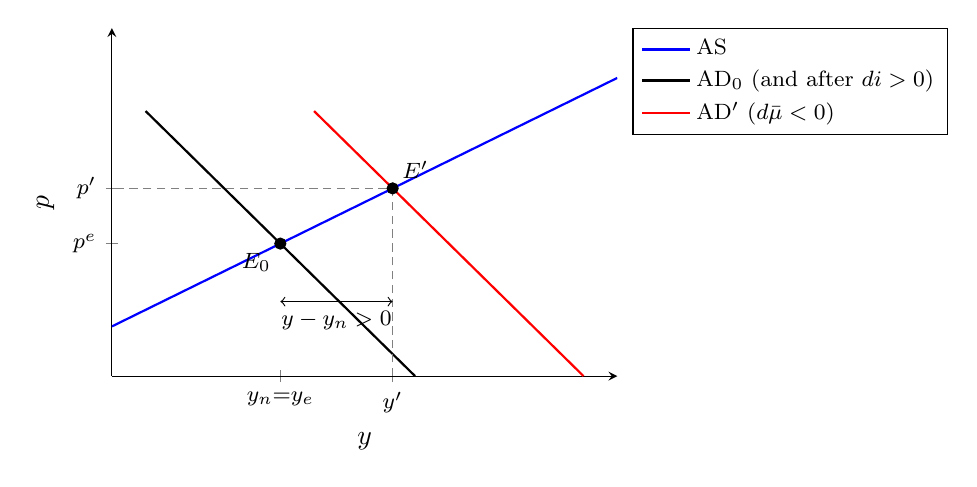
\begin{tikzpicture}
\begin{axis}[width=8cm,height=6cm,xmin=-1,xmax=2,ymin=-0.8,ymax=1.3,axis lines=left,xlabel={$y$},ylabel={$p$},
  xtick={0,0.6667},xticklabels={$y_n{=}y_e$,$y'$},ytick={0,0.3333},yticklabels={$p^e$,$p'$},
  tick label style={font=\footnotesize},legend style={font=\footnotesize},legend pos=outer north east,legend cell align=left]
\addplot[thick,blue,domain=-1:2]{0.5*x};
\addplot[thick,black,domain=-0.8:0.8]{-x};
\addplot[thick,red,domain=0.2:1.8]{-(x-1)};
\legend{AS,AD$_0$ (and after $di>0$),AD$'$ ($d\bar\mu<0$)}
\addplot[only marks,mark=*] coordinates {(0,0) (0.6667,0.3333)};
\node[font=\footnotesize,anchor=north east] at (axis cs:0,0) {$E_0$};
\node[font=\footnotesize,anchor=south west] at (axis cs:0.6667,0.3333) {$E'$};
\draw[gray,densely dashed] (axis cs:0.6667,-0.8) -- (axis cs:0.6667,0.3333) -- (axis cs:-1,0.3333);
\draw[<->] (axis cs:0,-0.35) -- (axis cs:0.6667,-0.35) node[midway,below,font=\footnotesize]{$y-y_n>0$};
\end{axis}
\end{tikzpicture}
\end{center}
{\footnotesize Drawn with $\sigma=1$, $\kappa=0.5$, $d\bar y=1$: $E'=(2/3,1/3)$ (check script). The rise $di=1$ moves AD$'$ back onto AD$_0$.}
\rubrica{
\item Curve and closed forms: 2 pts. Graph (scored on its own): axes, AS through $(y_n,p^e)$, AD$_0$, AD$'$, $E_0$, $E'$, gap: 2 pts.
}
\end{sol}

\textbf{c)} (2 points) In words: what changes if the news is a \emph{rise} in $\bar\mu$ (Prova 01, Q3)? Does the answer depend on $\phi$?
\resolespaco
\begin{sol}
\begin{notacao}
\item Symbols as in (a). Here $d\bar\mu>0$, $d\mu=0$. $\phi\ge0$: the weight on price surprises in the loss \eqref{LF}.
\end{notacao}
\passo{flip}{By \eqref{YB}, $d\bar y=-d\bar\mu/\Omega<0$, so every sign flips: AD left, $y$ and $p$ fall, $y-y_n<0$ and $y-y_e<0$. By \eqref{q2:di}
the bank \textbf{cuts} $i$:}
\begin{align}
di&=\frac{d\bar y}{\sigma}\nonumber\\
&=\frac{(-d\bar\mu/\Omega)}{\sigma}\nonumber\\
&=-\frac{d\bar\mu}{\sigma\Omega}<0 , \nonumber
\end{align}
at no cost. The AS does not move because current $\mu$ did not change. $\phi$ is irrelevant: neither $y_n$ nor $y_e$ moved, so the
optimum of the loss is the old point and the bank only undoes the AD shift (\eqref{q4:di} in Question 4(c)).
\refbib{Benigno (2015), \S6.3, Fig.\ 8, p.~513; \S4.2, p.~508 ($\bar\mu$ in $\bar y$); \texttt{Prova/prova-01-error-analysis.md}, Q3.}
\rubrica{\item AD left and a cut: 1 pt. ``AS moves'' or ``raise $i$'': 0 for the item. $\phi$-independence with the reason: 1 pt.}
\end{sol}

% -----------------------------------------------------------------------------
\questao{(10 points) \textit{Source: MPE Macroeconomics I, Lista 7 (2026), Question 2, item (a) only --- reproduced verbatim (its
points label and item (b) omitted); built also on Benigno, P. (2015), ``New-Keynesian Economics: An AS--AD View'', \S7, Fig.~9,
pp.~513--514, which has no exercises.}}

\noindent\textbf{Lista 7, Question 2.} Using separate AS--AD diagrams, analyze the following changes:
\begin{enumerate}[label=\alph*),leftmargin=2.2em,topsep=2pt,itemsep=1pt]
\item a temporary increase in firms' desired markups;
\end{enumerate}
In each case, identify which curve shifts, indicate the direction of the shift, and describe the effects on output and the price
level. Explain the economic intuition behind the movement of the curve and the resulting equilibrium.

\noindent What Benigno states (p.~513): ``This section considers only temporary mark-up shocks, leaving other analyses to the reader.''

\noindent\textit{Added parts (not in Lista 7), with the sign changed:} the desired markup \emph{falls} for one period only, $d\mu<0$
(a temporary payroll-tax cut, or a fall in the oil price); $d\bar\mu=0$. Items (a)--(c) below are this list's.

\textbf{a)} (3 points) With $i$ fixed: which curve moves and where; $dy$, $dp$, $d(y-y_n)$, $d(y-y_e)$ with signs.
\resolespaco
\begin{sol}
\begin{notacao}
\item $y$, $p$, $\bar y$, $p^e$, $y_n$, $y_e$, $i$, $\mu$, $\bar\mu$, $\sigma>0$, $\kappa>0$, $\Omega\equiv\sigma^{-1}+\eta>0$: as in Question~1.
\item The shock: $d\mu<0$ for one period, $d\bar\mu=0$.
\item $\phi\ge0$: weight on price surprises in \eqref{LF}. $y^*$, $p^*$, $i^*$: the bank's optimal output, price and rate.
\end{notacao}
\passo{curves}{Differentiate \eqref{YN} with only $\mu$ moving:}
\begin{equation}
dy_n=-\frac{d\mu}{\Omega}>0 . \label{q3:dyn}
\end{equation}
\eqref{YE} has no $\mu$, so $dy_e=0$; \eqref{YB} has no current $\mu$, so $d\bar y=0$. The AS shifts \emph{right} (down), through $(y_n',p^e)$;
by \eqref{q1:dAD} the AD stays.
\passo{solution}{Put only $dy_n$ in \eqref{q1:M} and divide by $1+\sigma\kappa$:}
\begin{equation}
d(y-y_n)=\frac{-dy_n}{1+\sigma\kappa}<0 . \label{q3:gap}
\end{equation}
Add $dy_n$ to \eqref{q3:gap}, as in \eqref{q1:dya}:
\begin{align}
dy&=dy_n+\Big(\frac{-dy_n}{1+\sigma\kappa}\Big)\nonumber\\
&=dy_n-\frac{dy_n}{1+\sigma\kappa}\nonumber\\
&=\frac{\sigma\kappa\,dy_n}{1+\sigma\kappa}>0 . \label{q3:dy}
\end{align}
By \eqref{q1:dAS} with $dp^e=0$, $dp=\kappa\,d(y-y_n)$. Substitute \eqref{q3:gap}:
\begin{align}
dp&=\kappa\Big(\frac{-dy_n}{1+\sigma\kappa}\Big)\nonumber\\
&=\frac{-\kappa\,dy_n}{1+\sigma\kappa}<0 . \label{q3:dp}
\end{align}
Since $dy_e=0$, $d(y-y_e)=dy>0$ by \eqref{q3:dy}. The two gaps have \emph{opposite} signs: output is below natural (so prices fall)
and above efficient.
\passo{confirmation}{This is the mirror image of Lista 7, Q2(a). The instructor's key (\texttt{Listas/solu\c{c}\~oes do instrutor/PSET 7 (1).pdf},
p.~1) shifts only the AS, to the left, with the AD fixed and $p'>p^e$; \texttt{Map/lista-07.md} (row 2a) gives $y\downarrow$, $p\uparrow$,
$y-y_n>0$, $y-y_e<0$. Reversing the sign of $d\mu$ reverses every entry, as above.}
\rubrica{\item AS only, right: 1 pt. AD shifted: max.\ 1 pt for the item. \item Closed forms: 1 pt. \item Two gaps with opposite signs: 1 pt; one ``output gap'': 0 for this line.}
\end{sol}

\textbf{b)} (3 points) Find the $di$ that keeps $p=p^e$ and the $di$ that keeps $y=y_e$. Report $y-y_e$ in the first case and $p-p^e$ in
the second. Is there a trade-off?
\resolespaco
\begin{sol}
\begin{notacao}
\item Symbols as in (a).
\end{notacao}
\passo{price stability}{Put $d(y-y_n)=0$ in \eqref{q1:M} with only $di$ and $dy_n$:}
\begin{equation}
0=-\sigma\,di-dy_n . \nonumber
\end{equation}
Solve for $di$ and substitute \eqref{q3:dyn}:
\begin{align}
di&=-\frac{dy_n}{\sigma}\nonumber\\
&=-\frac{(-d\mu/\Omega)}{\sigma}\nonumber\\
&=\frac{d\mu}{\sigma\Omega}<0 , \label{q3:dips}
\end{align}
a cut. Then $dy=dy_n$ and, since $dy_e=0$, $d(y-y_e)=dy_n>0$.
\passo{efficient output}{$y=y_e$ means $dy=0$. Put only $di$ and $dy_n$ in \eqref{q1:dy}:}
\begin{equation}
(1+\sigma\kappa)\,dy=\sigma\kappa\,dy_n-\sigma\,di . \nonumber
\end{equation}
Set $dy=0$ and solve for $di$:
\begin{equation}
di=\kappa\,dy_n>0 , \label{q3:die}
\end{equation}
a rise. By \eqref{q1:dAS} with $dy=0$:
\begin{equation}
dp=\kappa\,(0-dy_n)=-\kappa\,dy_n<0 . \nonumber
\end{equation}
\passo{trade-off}{\eqref{q3:dips} and \eqref{q3:die} have opposite signs: yes, a trade-off. The shock moves $y_n$ and not $y_e$.}
\rubrica{\item Each rate with sign and its outcome: 1 pt each. \item Trade-off traced to $y_n-y_e$: 1 pt.}
\end{sol}

\textbf{c)} (4 points) The bank minimizes $L$. Find $dy^*$, $dp^*$ and $di^*$, and the condition on $\phi$ under which it cuts.
\resolespaco
\begin{sol}
\begin{notacao}
\item Symbols as in (a); $y^*$, $p^*$, $i^*$ and $\phi$ as listed there.
\end{notacao}
\passo{optimum}{Question 4(a) gives the optimum \eqref{q4:ystar}. Differentiate it with $dy_e=0$:}
\begin{equation}
dy^*=\frac{\phi\kappa\,dy_n}{1+\phi\kappa}>0 . \label{q3:dys}
\end{equation}
By \eqref{q1:dAS} with $dp^e=0$, $dp^*=\kappa(dy^*-dy_n)$. Substitute \eqref{q3:dys}:
\begin{align}
dp^*&=\kappa\Big(\frac{\phi\kappa\,dy_n}{1+\phi\kappa}-dy_n\Big)\nonumber\\
&=\kappa\,\frac{\phi\kappa\,dy_n-(1+\phi\kappa)\,dy_n}{1+\phi\kappa}\nonumber\\
&=\frac{-\kappa\,dy_n}{1+\phi\kappa}<0 . \label{q3:dps}
\end{align}
\passo{rate}{Put $d\bar y=dg=d\bar g=d\bar p=0$ in \eqref{q1:dAD}:}
\begin{equation}
dy^*=-\sigma\,di^*-\sigma\,dp^* . \nonumber
\end{equation}
Solve for $di^*$:
\begin{equation}
di^*=-\frac{dy^*+\sigma\,dp^*}{\sigma}. \label{q3:di0}
\end{equation}
Add \eqref{q3:dys} and $\sigma$ times \eqref{q3:dps}:
\begin{align*}
dy^*+\sigma\,dp^*&=\Big(\frac{\phi\kappa\,dy_n}{1+\phi\kappa}\Big)+\sigma\Big(\frac{-\kappa\,dy_n}{1+\phi\kappa}\Big)\\
&=\frac{\phi\kappa\,dy_n-\sigma\kappa\,dy_n}{1+\phi\kappa}\\
&=\frac{\kappa(\phi-\sigma)\,dy_n}{1+\phi\kappa}.
\end{align*}
Substitute this into \eqref{q3:di0}:
\begin{align}
di^*&=-\frac{\Big(\frac{\kappa(\phi-\sigma)\,dy_n}{1+\phi\kappa}\Big)}{\sigma}\nonumber\\
&=-\frac{\kappa(\phi-\sigma)\,dy_n}{\sigma(1+\phi\kappa)}. \label{q3:dis}
\end{align}
\passo{sign}{By \eqref{q3:dyn}, $dy_n>0$. So in \eqref{q3:dis}, $di^*<0$ (cut) iff $\phi>\sigma$, and $di^*>0$ iff $\phi<\sigma$. Compare \eqref{q3:dps}
with the no-policy \eqref{q3:dp}: a hawk ($\phi>\sigma$) wants less price fall than the no-policy point gives
($\frac{1}{1+\phi\kappa}<\frac{1}{1+\sigma\kappa}$), so it pushes AD right.}
\refbib{Benigno (2015), \S7, Fig.\ 9, pp.~513--514; \S11, p.~522 (sign of the response depends on the IT slope); \texttt{Map/benigno/06-markup-shocks.md} \S6.3.}
\rubrica{\item $dy^*$, $dp^*$ from $dL/dy=0$ on AS: 2 pts. Optimisation in $i$ without AS: max.\ 1 pt for the item. \item $di^*$ and the $\phi\gtrless\sigma$ condition: 2 pts.}
\end{sol}

% -----------------------------------------------------------------------------
\questao{(10 points) \emph{Optimal policy.} \textit{Sources: MPE Macroeconomics I, Lista 7 (2026), Question 4 --- reproduced verbatim
(its points label omitted); Carlin, W. and Soskice, D. (2024), \emph{Macroeconomics: Institutions, Instability, and Inequality},
\S3.6.1 checklist questions 4 and 5, p.~156 --- reproduced verbatim; built also on Benigno, P. (2015), ``New-Keynesian Economics:
An AS--AD View'', \S11, eqs.~(33)--(35), Fig.~14, pp.~521--523, which has no exercises.}}

\noindent\textbf{Lista 7, Question 4.} The microeconomic foundations of the New Keynesian model make it possible to evaluate
monetary policy in terms of household welfare.

\noindent Consider the following loss function in conjunction with the AS-AD dynamics seen in Benigno (2015)
\begin{align*}
&\min_{y,p}\mathcal{L}=\phi_y(y-y^*)^2+\phi_p(p-p^e)^2, \qquad \phi_y,\phi_p>0,\\
&\text{s.t:}\\
&p-p^e=\kappa(y-y_n).
\end{align*}
Interpret the shape of the loss function and analyse what it implies for the behavior of a central bank. Also, explain why this
problem is subjected to the AS condition and what does that mean in terms of economic policy

\noindent\textbf{Carlin and Soskice, checklist questions 4 and 5.}
\begin{enumerate}[label=\arabic*.,leftmargin=2.2em,topsep=2pt,itemsep=1pt,start=4]
\item Explain what is meant by the central bank's loss function. How are the central bank's preferences reflected in the loss
function? Draw the loss `circles' for the cases where
\begin{enumerate}[label=(\alph*),topsep=1pt,itemsep=0pt]
\item $\beta=1$;
\item $\beta<1$;
\item $\beta>1$.
\end{enumerate}
In which of the three cases will the central bank reduce inflation back to target quickest after an inflation shock? Is there any
downside to adopting this policy stance?
\item Assume that $\alpha=\beta=1$, derive the $MR$ curve graphically using the tangencies between the loss circles and the Phillips
curves. With reference to the diagrams, explain the effect of the following (in each case, assume all other parameters are held
constant):
\begin{enumerate}[label=(\alph*),topsep=1pt,itemsep=0pt]
\item An increase in the slope of the Phillips curve, $\alpha$
\item An increase in central bank's inflation aversion, $\beta$.
\end{enumerate}
\end{enumerate}

\noindent What Benigno states (p.~522): ``This rule is robust to all types of shock and does not depend on their properties.''

\noindent\textit{Added parts (not in the sources):} items (a)--(c) below are this list's. They ask the questions above in Benigno's
static model and with the loss $L$ of the cover: $\phi$ plays the role of Carlin and Soskice's $\beta$, $\kappa$ of their $\alpha$, the
IT line of their $MR$ curve.

\textbf{a)} (4 points) Minimize $L$ subject to the AS. Derive the targeting rule, explain why the AS (and not the AD) is the constraint,
and describe the loss contours and the IT line. Show that the Lista 7 loss $\phi_y(y-y^*)^2+\phi_p(p-p^e)^2$ gives the same rule for suitable weights.
\resolespaco
\begin{sol}
\begin{notacao}
\item $y$, $p$: log output and price level. $y_n$, $y_e$: natural and efficient output, \eqref{YN} and \eqref{YE}. $p^e$: preset price.
\item $\kappa>0$: slope of \eqref{AS}. $\phi\ge0$: weight on price surprises in the loss $L$ \eqref{LF}. $\sigma>0$, $i$: as in Question~1.
\item $y^*$: the optimal output (in this question). $c>0$: a level of the loss, $L=c$ (a contour).
\item IT line: the targeting rule drawn in the $(y,p)$ plane.
\item Lista 7 loss only: $L_7\equiv\phi_y(y-y^*)^2+\phi_p(p-p^e)^2$; $\phi_y,\phi_p>0$ are its weights and $y^*$ there is that list's output target, not the optimum.
\end{notacao}
\passo{substitution}{Square both sides of \eqref{AS}:}
\begin{equation}
(p-p^e)^2=\kappa^2(y-y_n)^2 . \label{q4:sq}
\end{equation}
Substitute \eqref{q4:sq} into the second term of \eqref{LF}:
\begin{align}
L&=\tfrac12(y-y_e)^2+\tfrac{\phi}{2\kappa}\,\big(\kappa^2(y-y_n)^2\big)\nonumber\\
&=\tfrac12(y-y_e)^2+\tfrac{\phi\kappa}{2}(y-y_n)^2 . \label{q4:Ly}
\end{align}
\passo{FOC}{Differentiate \eqref{q4:Ly} with respect to $y$ and set it to zero:}
\begin{equation}
\frac{dL}{dy}=(y-y_e)+\phi\kappa\,(y-y_n)=0 . \label{q4:foc}
\end{equation}
Differentiate once more: $\frac{d^2L}{dy^2}=1+\phi\kappa>0$, so \eqref{q4:foc} gives a minimum. By \eqref{AS}, $\kappa(y-y_n)=p-p^e$; substitute
this into \eqref{q4:foc}:
\begin{equation}
(y-y_e)+\phi\,(p-p^e)=0 . \label{q4:rule}
\end{equation}
Collect the $y$ terms of \eqref{q4:foc}:
\begin{equation}
y\,(1+\phi\kappa)=y_e+\phi\kappa\,y_n . \nonumber
\end{equation}
Divide by $1+\phi\kappa$:
\begin{equation}
y^*=\frac{y_e+\phi\kappa\,y_n}{1+\phi\kappa}. \label{q4:ystar}
\end{equation}
\passo{why AS}{$i$ enters only \eqref{AD}, and by \eqref{q1:dAD} a change in $i$ shifts the AD horizontally by $-\sigma\,di$: any point of the
AS can be reached. The AD restricts nothing; the AS (firms' price setting) is the menu of $(y,p)$ the bank can choose from.}
\passo{geometry}{Set \eqref{LF} equal to $c$ and divide by $c$:}
\begin{equation}
\frac{(y-y_e)^2}{2c}+\frac{(p-p^e)^2}{2c\kappa/\phi}=1 , \nonumber
\end{equation}
an ellipse centred at $(y_e,p^e)$ (a circle iff $\phi=\kappa$). The optimum is the tangency of the lowest ellipse with the AS. Solve
\eqref{q4:rule} for $p$:
\begin{equation}
p-p^e=-\frac1\phi\,(y-y_e) , \label{q4:IT}
\end{equation}
the IT line: slope $-1/\phi$, through $(y_e,p^e)$.
\passo{Lista 7}{Substitute \eqref{q4:sq} into the Lista 7 loss:}
\begin{equation}
L_7=\phi_y(y-y^*)^2+\phi_p\big(\kappa^2(y-y_n)^2\big) . \nonumber
\end{equation}
Differentiate with respect to $y$, set it to zero and divide by 2:
\begin{equation}
\phi_y(y-y^*)+\phi_p\kappa^2(y-y_n)=0 . \nonumber
\end{equation}
Replace $\kappa(y-y_n)$ by $p-p^e$ using \eqref{AS}:
\begin{equation}
\phi_y(y-y^*)+\kappa\phi_p(p-p^e)=0 , \label{q4:rule7}
\end{equation}
the rule in \texttt{Map/lista-07.md} (Q4). Put $\phi_y=\frac12$, $\phi_p=\frac{\phi}{2\kappa}$, $y^*=y_e$ in \eqref{q4:rule7}:
\begin{align}
\big(\tfrac12\big)\big(y-(y_e)\big)+\kappa\big(\tfrac{\phi}{2\kappa}\big)(p-p^e)&=0\nonumber\\
\tfrac12(y-y_e)+\tfrac\phi2(p-p^e)&=0 , \nonumber
\end{align}
which is \eqref{q4:rule} divided by 2. (The instructor's PSET 7 key does not cover Q4; the check is against the project's verified answer.)
\rubrica{\item Substitution of AS and $dL/dy=0$ with SOC: 2 pts. Differentiating in $i$ or using a $y_e$ that contains $\mu$ (Prova 01, 3.c): max.\ 1 pt.
\item Why AS, contours and IT line: 1.5 pts. \item Lista 7 mapping: 0.5 pt.}
\end{sol}

\textbf{b)} (3 points) Let $W\equiv y_e-y_n>0$. Find $y^*-y_e$ and $p^*-p^e$, sign their derivatives in $\phi$ and $\kappa$, and give the limits
$\phi\to\infty$ and $\phi=0$. Relate the answer to the two Carlin--Soskice questions.
\resolespaco
\begin{sol}
\begin{notacao}
\item Symbols as in (a). New: $W\equiv y_e-y_n>0$, the wedge between efficient and natural output. $p^*$: the optimal price level.
\item $\partial_\phi$, $\partial_\kappa$: partial derivatives with respect to $\phi$ and $\kappa$.
\end{notacao}
\passo{levels}{Subtract $y_n$ from \eqref{q4:ystar}:}
\begin{align}
y^*-y_n&=\frac{y_e+\phi\kappa\,y_n-(1+\phi\kappa)\,y_n}{1+\phi\kappa}\nonumber\\
&=\frac{y_e-y_n}{1+\phi\kappa}\nonumber\\
&=\frac{W}{1+\phi\kappa}. \label{q4:gapn}
\end{align}
Subtract $W=y_e-y_n$ from \eqref{q4:gapn}:
\begin{align}
y^*-y_e&=\frac{W}{1+\phi\kappa}-W\nonumber\\
&=-\frac{\phi\kappa\,W}{1+\phi\kappa}. \label{q4:gape}
\end{align}
By \eqref{AS}, $p^*-p^e=\kappa(y^*-y_n)$. Substitute \eqref{q4:gapn}:
\begin{align}
p^*-p^e&=\kappa\Big(\frac{W}{1+\phi\kappa}\Big)\nonumber\\
&=\frac{\kappa W}{1+\phi\kappa}. \label{q4:pgap}
\end{align}
\passo{derivatives}{Differentiate \eqref{q4:pgap} with respect to $\phi$:}
\begin{equation}
\partial_\phi(p^*-p^e)=-\frac{\kappa^2W}{(1+\phi\kappa)^2}<0 . \nonumber
\end{equation}
Differentiate \eqref{q4:pgap} with respect to $\kappa$ (quotient rule):
\begin{align*}
\partial_\kappa(p^*-p^e)&=\frac{(1+\phi\kappa)-\phi\kappa}{(1+\phi\kappa)^2}\,W\\
&=\frac{W}{(1+\phi\kappa)^2}>0 .
\end{align*}
Differentiate \eqref{q4:gape} with respect to $\phi$ and to $\kappa$:
\begin{align*}
\partial_\phi(y^*-y_e)&=-\frac{\kappa W}{(1+\phi\kappa)^2}<0 ,\\
\partial_\kappa(y^*-y_e)&=-\frac{\phi W}{(1+\phi\kappa)^2}<0 .
\end{align*}
\passo{limits}{Let $\phi\to\infty$ in \eqref{q4:gapn} and \eqref{q4:pgap}: $y^*\to y_n$, $p^*\to p^e$ (strict price stability). Put $\phi=0$ in
\eqref{q4:gape} and \eqref{q4:pgap}: $y^*=y_e$, $p^*-p^e=\kappa W$.}
\passo{Carlin--Soskice}{More inflation aversion ($\phi$, their $\beta$) flattens the IT/MR line \eqref{q4:IT} (slope $-1/\phi$): less of the
wedge into prices, more into output.
A steeper AS ($\kappa$, their $\alpha$) makes each unit of output above $y_n$ cost more price surprise.}
\rubrica{\item Levels: 1 pt. \item Four signed derivatives: 1 pt. \item Limits and the analogy: 1 pt.}
\end{sol}

\textbf{c)} (3 points) For a shock with changes $dy_n$, $dy_e$, $d\bar y$ ($g$, $\bar p$, $p^e$ fixed), find $di^*$ and prove that it depends on $\phi$
if and only if $dy_n\neq dy_e$. Apply the result to news of a higher $\bar\mu$.
\resolespaco
\begin{sol}
\begin{notacao}
\item Symbols as in (a) and (b). $dy_n$, $dy_e$, $d\bar y$: the shock's changes in natural, efficient and long-run output.
\item New: $X\equiv dy_e-dy_n$, the change in the wedge $W$. $i^*$: the optimal rate. $\Omega\equiv\sigma^{-1}+\eta$, $\bar\mu$: as in Question~1.
\end{notacao}
\passo{optimum}{Differentiate \eqref{q4:ystar}:}
\begin{equation}
dy^*=\frac{dy_e+\phi\kappa\,dy_n}{1+\phi\kappa}. \label{q4:dys}
\end{equation}
Write $dy_n=dy_e-X$ in \eqref{q4:dys}:
\begin{align}
dy^*&=\frac{dy_e+\phi\kappa\,(dy_e-X)}{1+\phi\kappa}\nonumber\\
&=\frac{(1+\phi\kappa)\,dy_e-\phi\kappa X}{1+\phi\kappa}\nonumber\\
&=dy_e-\frac{\phi\kappa X}{1+\phi\kappa}. \label{q4:dys2}
\end{align}
By \eqref{q1:dAS} with $dp^e=0$, $dp^*=\kappa(dy^*-dy_n)$. From \eqref{q4:dys}, $dy^*-dy_n=\frac{dy_e-dy_n}{1+\phi\kappa}=\frac{X}{1+\phi\kappa}$, so
\begin{align}
dp^*&=\kappa\Big(\frac{X}{1+\phi\kappa}\Big)\nonumber\\
&=\frac{\kappa X}{1+\phi\kappa}. \label{q4:dps}
\end{align}
\passo{rate}{Put $dg=d\bar g=d\bar p=0$ in \eqref{q1:dAD}:}
\begin{equation}
dy^*=d\bar y-\sigma\,di^*-\sigma\,dp^* . \nonumber
\end{equation}
Solve for $di^*$:
\begin{equation}
di^*=\frac{d\bar y-dy^*-\sigma\,dp^*}{\sigma}. \label{q4:di0}
\end{equation}
Add \eqref{q4:dys2} and $\sigma$ times \eqref{q4:dps}:
\begin{align}
dy^*+\sigma\,dp^*&=\Big(dy_e-\frac{\phi\kappa X}{1+\phi\kappa}\Big)+\sigma\Big(\frac{\kappa X}{1+\phi\kappa}\Big)\nonumber\\
&=dy_e+\frac{(\sigma-\phi)\,\kappa X}{1+\phi\kappa}. \nonumber
\end{align}
Substitute this into \eqref{q4:di0}:
\begin{align}
di^*&=\frac{d\bar y-\Big(dy_e+\frac{(\sigma-\phi)\,\kappa X}{1+\phi\kappa}\Big)}{\sigma}\nonumber\\
&=\frac{d\bar y-dy_e}{\sigma}-\frac{(\sigma-\phi)\,\kappa X}{\sigma(1+\phi\kappa)}. \label{q4:di}
\end{align}
\passo{proof}{Only the last term of \eqref{q4:di} contains $\phi$. Differentiate its $\phi$ part (quotient rule):}
\begin{align*}
\frac{\partial}{\partial\phi}\,\frac{-(\sigma-\phi)}{1+\phi\kappa}&=\frac{(1+\phi\kappa)+(\sigma-\phi)\kappa}{(1+\phi\kappa)^2}\\
&=\frac{1+\sigma\kappa}{(1+\phi\kappa)^2}.
\end{align*}
Multiply by $\frac{\kappa X}{\sigma}$:
\begin{equation}
\frac{\partial di^*}{\partial\phi}=\frac{\kappa(1+\sigma\kappa)\,X}{\sigma(1+\phi\kappa)^2}, \label{q4:ddi}
\end{equation}
zero iff $X=0$. With $X=0$, $dy_e=dy_n$; substitute both into \eqref{q4:di}:
\begin{align}
di^*&=\frac{d\bar y-(dy_n)}{\sigma}-\frac{(\sigma-\phi)\,\kappa\,(0)}{\sigma(1+\phi\kappa)}\nonumber\\
&=\frac{d\bar y-dy_n}{\sigma}, \nonumber
\end{align}
the strict price-stability rate (\eqref{q1:M} with $d(y-y_n)=0$).
\passo{$\bar\mu$ news}{By \eqref{YN} and \eqref{YE}, $dy_n=dy_e=0$, so $X=0$; by \eqref{YB}, $d\bar y=-\frac{d\bar\mu}{\Omega}$. Substitute into \eqref{q4:di}:}
\begin{align}
di^*&=\frac{(-d\bar\mu/\Omega)-(0)}{\sigma}-\frac{(\sigma-\phi)\,\kappa\,(0)}{\sigma(1+\phi\kappa)}\nonumber\\
&=-\frac{d\bar\mu}{\sigma\Omega}<0 \nonumber
\end{align}
for every $\phi$, as in Prova 01, 3.c (error analysis, Q3).
\intuicao{$\phi$ chooses a point on the AS only when the shock separates $y_n$ from $y_e$; otherwise the best point is unique and the
bank just moves AD back to it.}
\rubrica{\item $di^*$ in closed form: 1.5 pts. \item Proof of the iff: 1 pt. \item Application, with ``cut, for any $\phi$'': 0.5 pt.}
\end{sol}
